%%%%%%%%%%%%%%%%%%%%%%%%%%%%%%%%%%%%%%%%%
% Diaz Essay
% LaTeX Template
% Version 2.0 (13/1/19)
%
% This template originates from:
% http://www.LaTeXTemplates.com
%
% Authors:
% Vel (vel@LaTeXTemplates.com)
% Nicolas Diaz (nsdiaz@uc.cl)
%
% License:
% CC BY-NC-SA 3.0 (http://creativecommons.org/licenses/by-nc-sa/3.0/)
%
%%%%%%%%%%%%%%%%%%%%%%%%%%%%%%%%%%%%%%%%%

%----------------------------------------------------------------------------------------
%	PACKAGES AND OTHER DOCUMENT CONFIGURATIONS
%----------------------------------------------------------------------------------------

\documentclass[11pt]{diazessay} % Font size (can be 10pt, 11pt or 12pt)
\usepackage[export]{adjustbox}
\usepackage{subcaption}
%----------------------------------------------------------------------------------------
%	TITLE SECTION
%----------------------------------------------------------------------------------------

\title{\textbf{Report} \\ {\Large\itshape Doggos emotions recognition and classification}} % Title and subtitle

\author{\textbf{Artificial Inteligence} \\ \textit{Anna Przybycien, Agnieszka Szlendak}} % Author and institution

\date{\today} % Date, use \date{} for no date

%----------------------------------------------------------------------------------------

\begin{document}

\maketitle % Print the title section

%----------------------------------------------------------------------------------------
%	ABSTRACT AND KEYWORDS
%----------------------------------------------------------------------------------------

%\renewcommand{\abstractname}{Summary} % Uncomment to change the name of the abstract to something else

\begin{abstract}
Nowadays, there are plenty of machine learning projects focused on image recognition and caption generation. Great chunk of it is about recognizing human face and naming emotion it express. We decided to build image recognition with emotion capture, not for human faces though, but for dog's muzzles, as there is no good model to do that yet and far more fun.
\end{abstract}

%\hspace*{3.6mm}\textit{Keywords:} emotion recognition, CNN, doggos, wisdom, %knowledge, hudge mess, majnas % Keywords

\vspace{10pt} % Vertical whitespace between the abstract and first section

%----------------------------------------------------------------------------------------
%	ESSAY BODY
%----------------------------------------------------------------------------------------

\section*{Task description}

Our task consists of two major parts:

\begin{itemize}
	\item prepartion:

	\begin{itemize}
		\item create a dataset of dogs photos
		\item tag photos with proper emotions
	\end{itemize}

	\item AI implementation:
	\begin{itemize}
		\item find doggo on the photo (detect the doggo's muzzle)
		\item recognise the emotion (from a set of possible emotions, assess what is express on the image)
	\end{itemize}

\end{itemize}
%------------------------------------------------


\section*{Common approaches}

Preparation of proper dataset is crucial for all machine learning projects. Common practise is to take pre-existing sets of data prepared specially for the machine learning tasks (MIT datasets/kaggle datasets). If there is no dataset avaible for the task, one must create it oneself. For image datasets, it is done by finding database of pictures and then use the tagger. There are plenty of existing taggers on the Internet, but provided that none is suited for the type of the task, one should create a tagger himself.

Computer vision is rapidly growing interdisciplinary field, that deals with computers gaing understanding from photos. In our research, we focused on two topics, mainly: how human emotion recognition from pictures is done and how can it be applied to captioning doggo's emotion (is it possible).

In this type of tasks (workin with pictures, recognizing what's on them) neural networks are the most useful. They are ones of the most popular machine learning algorithms at present and are proven to outperform other algorithms in accuracy and speed. 
In recent scientific papers, two types of neural networks seem to be the most popular: 
\begin{itemize}
	\item CNN (Convolutional Neutral Network) - it derives its name from the type of hidden layers it consists of - convolutional layers, pooling layers, fully connected layers, and normalization layers. An input is processed through them and an output is produced, with an assumption that two successive inputs are independent of each other. 
Convolution and pooling functions are used as activation functions (functions that are applied to an input of the neuron) (example in usage: Deep Face)
	
\begin{center}%{l}{1\textwidth} % Inline image example, use an 'r' column type to position the figure on the right
	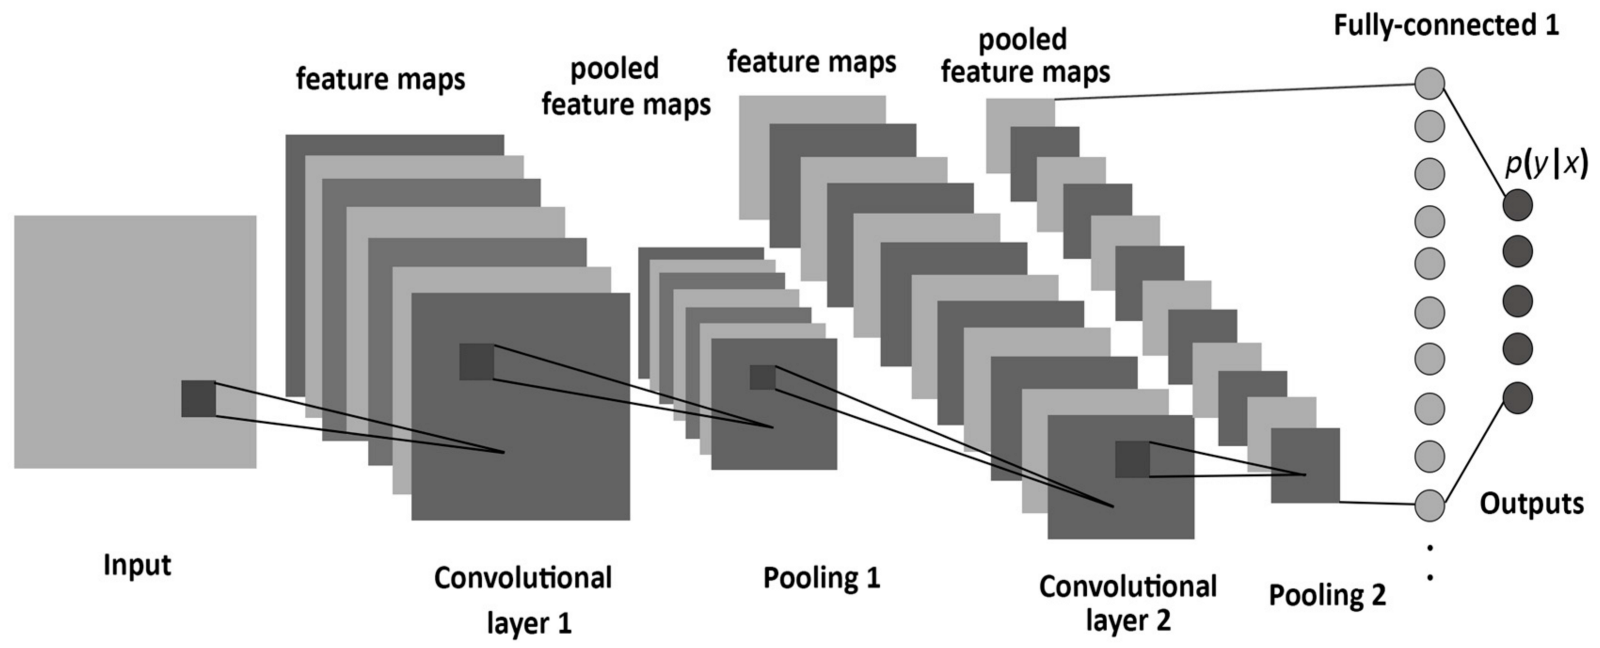
\includegraphics[scale=0.2]{cnn.png}
%	\caption{An example fish.}
\end{center}

	\item RNN (Recursive Neural Network) - this variation of the network allows two successive inputs to be dependent of each other - as it happend very often in real life.
	
It performs the same task for every element of a sequence, with the output being depended on the previous computations. Another way to think about RNNs is that they have a “memory” which captures information about what has been calculated so far.
\end{itemize}

%------------------------------------------------

\section*{Our solution}
To tackle the problem with no pre-existing dataset, we would prepare it using:
	\begin{itemize}
		\item tagger: 
			\begin{itemize}
				\item https://github.com/Microsoft/VoTT
			\end{itemize}
		\item photos from Instagram Api: 
			\begin{itemize}
				\item https://www.instagram.com/explore/tags/dogsofinstagram/
			\end{itemize}
		
	\end{itemize}
Tagger will enable us to mark the dog's muzzle and name the emotion it's expressing.

We are yet to decide whether we want to just named the emotions or use arousal - valence scale suited for doggo's emotions (so each photo will be tagged with two values x, y representing score on the according axis).
  
\begin{center}%{l}{1\textwidth} % Inline image example, use an 'r' column type to position the figure on the right
	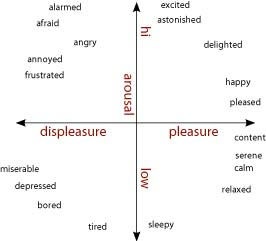
\includegraphics[scale=0.6]{emotion-scale.jpg}
%	\caption{An example fish.}
\end{center}

Our choice of algorithm is now settled on Convolution Neural Network, for a couple of reasons: it is better suited for our's type of task (CNN can be stacked into a very deep model, which has been proven to be very effective in capturing features. On the contrary, due to the gradient vanishing and exploding problems, RNN models are usually very shallow, 2 or 3 layers), we had experience with building CNN from another project, we can head start our project by taking pre-trained model, such as deep fake and cutting last layers of CNN (as they are the most detailed) to check whether learing emotion recognition in humans can be used to recognize doggo's emotions.

We will procede to represent out images as matrixes of pixels with 3 values for color (RGB) - enables our later algorithm to read them and learn from them. 
To train our model, we will use the algorithm that consists of convolutional layers that will detect patters. It will be done by matrix multiplication of the part of an image matrix with filter, then applying activating function - ReLu, polling layers that will generalize and minimize the size of the image (matrix) by taking maximum value of the pixel or the average of the chunk. In the end, fully connected layer will classify processed matrixes with the output being the name of the emotion or values for valence-arousal scale (which can be easily interpreted with names of emotions). 
After classification, we can compute loss function and bearing in mind those values adjust the filters and improve our algorithm.


%\hspace*{3.6mm}\textit{Keywords:} emotion recognition, CNN, doggos, wisdom, %knowledge, hudge mess, majnas % Keywords

\vspace{10pt} % Vertical whitespace between the abstract and first section

%----------------------------------------------------------------------------------------
%	ESSAY BODY
%----------------------------------------------------------------------------------------

\section*{Data preparation}
In order to create a model for classification we needed proper dataset with dogs images. Unfortunatelly, for now, there is no proper dataset published suited for dogs emotion recognition. We were faced with the challenge of creating the dataset by ourselfes. The task consisted of four major parts:
\begin{enumerate}
	\item Finding the data source. \\
	As downloading images manually from google graphics would be too much of a hussle, we decided to use a tool 4K Stogram, which enabled us to download pictures based on tags from Instagram directly on our discs.
	\\
	\item Defining number and characteristics of classes. \\ 
	Because of the time and resource access constraint, we had to limit the number of classes to four. We also vaguely assumed what are the characteristics of each class:
	\begin{itemize}
		\item \textbf{happy dogs} - dogs with the smile, mainly with open muzzle and tongue out
		\item \textbf{angry dogs} - dogs that looks scary, with their teeth showing
		\item \textbf{sleepy dogs} - dogs that are taking a nap, or are about to, with closed or squinted eyes,
		\item \textbf{good dogs} - dogs that looks polite, with neutral muzzle \\
	\end{itemize} 
	\item Determining classes numerousity \& dataset creation. \\ 
	First, we assume that minimum number of images for each class should be 500. We began dataset preparation with the phrase 'the bigger the better' in mind, but we were able only to reach our assumed baseline of 500 per class.
	So, from that point forward, we had dataset of 2000 classified images.\\
	\item Seperating into train, validation and test sets.\\ 
	Lastly, as our dataset was small, we proceed to separate it using 60/20/20 proportion:
	\begin{itemize}
		\item 60\% - 1200 (300 per class) images in training set
		\item 20\% - 400 (100 per class) images in validation set
		\item 20\% - 400 (100 per class) images in test set
	\end{itemize}
	
\end{enumerate}
\section*{AI implementation}
\begin{itemize}

	\item pure CNN \\
We started with the simplest neural network we could think of, one consisting of four layers - every one used relu as its activation function - and one with softmax at the end. \\We went for 30 epochs and achieved 30\% accuracy on validation data. Despite tremendous overitting we were off to a good start.  
	\item CNN with data augmentation \\
Overfitting was due to small size of our dataset, but it turned out that keras has perfect solution for it - easy to implement data augumentation - process that from one sample creates more by subjecting ir to various transformations. \\
This time we decided on 100 epochs, so after some time (even using GPU) we got 56\% accuracy with overfitting at smaller scale.   
	\item CNN with convolutional base taken from 'imagenet' \\
	To counter overfitting resulting from using small dataset, we decided to use transfer learning and introduce convolutional base, pre-trained on famous imagenet dataset. Imagenet includes pictures of all sorts of animals, including various breeds of dogs, so we cocluded it would be suitable for our needs. It performed much better than pure version, with ~60\% accuracy and similar to the version with data augmentation.
	\begin{figure}[h]
 
	\begin{subfigure}{0.5\textwidth}
    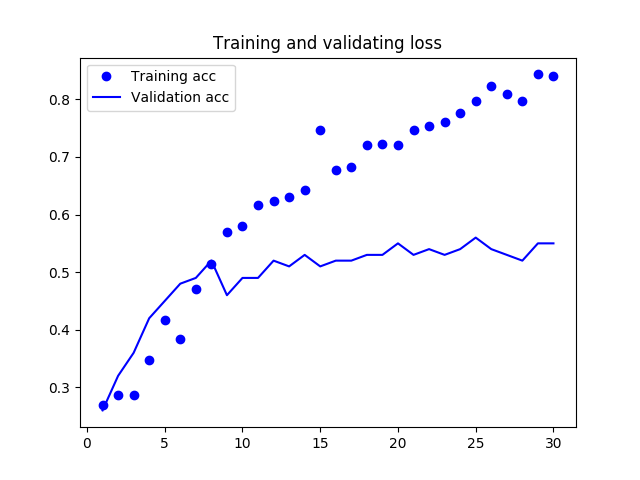
\includegraphics[scale=0.4, left]{cnn-imgenet-acc.png}
    \caption{Accuracy function}
    \label{fig:subim1}
    \end{subfigure}
    \begin{subfigure}{0.5\textwidth}
	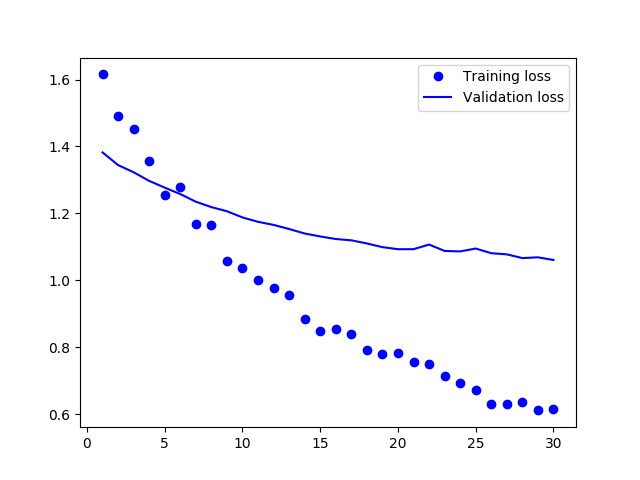
\includegraphics[scale=0.4, right]{cnn-imgenet-loss.png}
    \caption{Loss function}
    \label{fig:subim2}
    \end{subfigure}
 
    \caption{Accuracy and loss functions for CNN with 'imagenet'}
    \label{fig:image2}
    \end{figure}
	
	
    
	\item CNN with convolutional base taken from 'imagenet' with data augmentation and early stopping\\
	
\end{itemize}
%------------------------------------------------


\section*{Final remarks}

%\begin{center}%{l}{1\textwidth} % Inline image example, use an 'r' column type to position the figure on the right
%	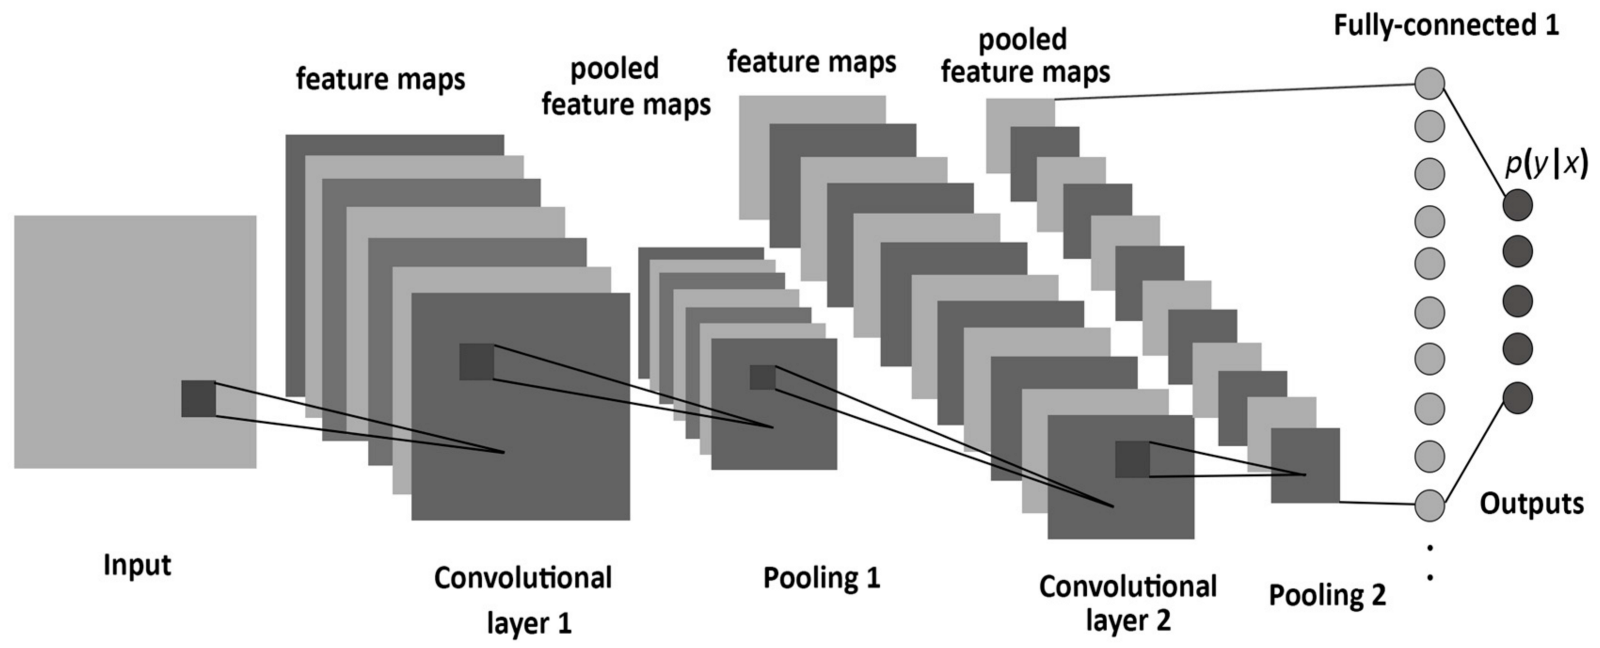
\includegraphics[scale=0.2]{cnn.png}
%	\caption{An example fish.}
%\end{center}


%------------------------------------------------

%----------------------------------------------------------------------------------------
%	BIBLIOGRAPHY
%----------------------------------------------------------------------------------------
\section*{Sources}
\begin{itemize}
\item
  \textit{Deep Learining with Python}, Fracouis Chollet.
\end{itemize}

%----------------------------------------------------------------------------------------

\end{document}
